\documentclass{vorkurs}
\usepackage[utf8]{inputenc}
\usepackage[T1]{fontenc}

\usepackage{xspace}
\usepackage[pass]{geometry}
\usepackage{tikz}
\usetikzlibrary{arrows,decorations.pathmorphing,decorations.footprints,fadings,calc,trees,mindmap,shadows,decorations.text,patterns,positioning,shapes,matrix,fit}
\usepackage{enumitem}
\usepackage{url}
\usepackage[pdftex,bookmarks=true,bookmarksnumbered=true,bookmarksopen=true,colorlinks=true,filecolor=black,
    linkcolor=red,urlcolor=blue,plainpages=false,pdfpagelabels,citecolor=black,
    pdftitle={Programmiervorkurs der Fachschaft
    MathPhys},setpagesize=false,pdfauthor={Axel Wagner}]{hyperref}

\newcommand{\swname}[1]{\texttt{#1}\xspace}
\newcommand{\Cpp}{\swname{C++}}
\newcommand{\Java}{\swname{Java}}
\newcommand{\Eclipse}{\swname{Eclipse}}
\newcommand{\file}[1]{\texttt{#1}\xspace}
\newcommand{\param}[1]{\texttt{#1}\xspace}

\begin{document}

Um Lesbarkeit zu gewährleisten, nutzt dieses Schriftstück das generische
Femininum.

Soweit personenbezogene Bezeichnungen in weiblicher Form aufgeführt sind,
beziehen sie sich auf alle Geschlechter in gleicher Weise.

\clearpage

\chapter*{Vorwort}
\pagestyle{empty}

Der vorliegende Einführungskurs in das prozedurale Programmieren wurde
ursprünglich von der Fachschaft
MathPhys\footnote{\url{https://mathphys.fsk.uni-heidelberg.de}} der Universität
Heidelberg entworfen. Er wurde 2017 von Fabian
Grünig\footnote{\texttt{gruenig@posteo.de}} für das Studienvorbereitungsprogramm
„Semester Null“ der DHBW Mosbach in die Programmiersprace \Java übersetzt und
auf die spezifischen Anforderungen dieses Programms angepasst.

Gedacht ist dieser Kurs für Menschen, die ihren Computer bisher eher zum
Spielen, als zum Arbeiten benutzt haben, die schon mal gehört haben, dass man
„Programmieren“ kann, sich darunter aber einen magischen Prozess vorstellen, den
nur Eingeweihte beherrschen und von dem man eigentlich lieber die Finger lässt,
wenn man nicht will, dass einem der Computer um die Ohren fliegt. Kurzum: Dieser
Kurs richtet sich an blutigste Anfängerinnen.

Wir wollen zeigen, dass Programmieren eigentlich gar nicht so schwer ist und
dass einem der Computer eigentlich viel mehr Spaß bringt, wenn man mit dem
nötigen Spieltrieb herangeht. Am Ende dieses Kurses sollte die Angst vor dem
Computer verflogen sein. Ihr solltet gesehen haben, dass es keinen Grund gibt,
ewig zu rätseln, ob ein Algorithmus nun korrekt ist und was die richtige Syntax
für eine Operation ist, statt einfach etwas hinzuschreiben und zu sehen, ob es
kompiliert und läuft. Die wichtigste Kompetenz, die wir Euch vermitteln wollen
ist, programmieren zu lernen, also zu wissen, wie man eine Fehlermeldung liest,
wo man bei Wissenslücken nachschauen kann und wen man fragen kann, wenn man mal
nicht weiter weiß.

Um diese Ziele zu erreichen, haben wir den Kurs aufgeteilt in viele kleine
Lektionen. Jede Lektion stellt im Wesentlichen eine abgeschlossene Einheit dar,
die eigenständig (mit bedarfsorientierter Hilfestellung) bearbeitet werden
sollen. Primär geht es dabei nicht um den dargestellten Inhalt, sondern darum,
mit diesem herumzuspielen und selbst die „Cornercases“ zu entdecken.
Insbesondere solltet ihr die Lektionen also \emph{nicht} unter künstlichem
Zeitdruck bearbeiten. Das Ziel ist es nicht, jede Lektion bearbeitet zu haben,
sondern jede Lektion \emph{entdeckt} zu haben. Selbstverantwortliches Lernen ist
tragender Gedanke des Kurses und sollte entsprechend ernst genommen werden;
entscheidet selbst, wie viel Zeit Ihr in welche Lektionen stecken wollt.

Jede Lektion gliedert sich wiederum in drei Teile:
\begin{enumerate}
\item Ein theoretischer Teil, in dem ein Unterbau für die Lektion gegeben werden
  soll. Ein tiefes Verständnis sollte für die Bearbeitung der Lektion nicht
  notwendig sein, es geht mehr darum, dass sich ein grober
  Wiedererkennungseffekt einstellt, wenn die theoretischen Kenntnisse im
  nächsten Teil vertieft werden.

  Wenn du einen eher passiven Lernstil pflegst, kannst du dir hier auch Deine
  Dozentin oder Deinen Dozenten bitten, dass sie Dich kurz in das Thema
  einführt.
\item Dem Theorieteil schließt sich der Praxisteil an. Hier soll selbstständig
  das eben hoffentlich oberflächlich Verstandene in einer kurzen Fingerübung
  angewendet werden.

  Bei Fragen kann man aber natürlich auch hier die Dozentin oder den Dozenten zu
  Rate ziehen.
\item Abschließend zu jeder Lektion steht dann ein „Spielteil“. Hier soll das
  Gelernte vertieft und „bespielt“ werden. Tiefer gehende Informationen werden
  vermittelt und Möglichkeiten, mit dem Code zu interagieren, aufgezeigt.

  Von diesem Teil sollte man sich am Wenigsten aufhalten, verunsichern oder
  deprimieren lassen.
\end{enumerate}

Als Sprache für den Kurs haben wir
\Java\footnote{\url{http://www.oracle.com/technetwork/java/index.html}} gewählt
und verwenden als Entwicklungsumgebung
\Eclipse\footnote{\url{https://www.eclipse.org/}}. Diese Umgebung stellt
vergleichsweise hohe Anforderungen an Anfängerinnen, da \Java in Kombination mit
\Eclipse eigentlich für große Projekte gedacht ist.

Der Grund, aus dem wir trotzdem \Java und \Eclipse einsetzen, ist, dass diese
Umgebung eine der am Weitesten verbreiteten Arbeitsumgebungen ist und für
Projekte im „Business“-Umfeld der übliche Standard ist. Außerdem wird \Java im
Studium an der DHBW Mosbach relevant und wir wollen Euch die Verwirrung
ersparen, direkt zu Beginn des Lernprozesses mit zwei verschiedenen Sprachen
oder Entwicklungsmgebungen konfrontiert zu werden.

%% Der gesamte Kurs ist aufgeteilt in mehrere Kapitel. Dies dient dem Zweck,
%% verschiedenste Bedürfnisse und Lerntempi zu befriedigen. Wer sich ganz auf die
%% Grundlagen konzentrieren und sich mit diesen intensiv auseinandersetzen möchte,
%% findet in den ersten Kapiteln Material, spielerisch die Sprache zu entdecken.
%% Wer sich im ersten Kapitel relativ wohl fühlt, ist bereits bestens auf die
%% Einführung auf ein „Informatik“-nahes Studium vorbereitet. Wer schneller lernt,
%% oder einen tieferen Einblick wünscht, findet in späteren Kapiteln genug
%% Material, um sich trotzdem zu beschäftigen und voll in die Sprache einzusteigen.

Abschließend sollte noch ein weiteres Mal einmal betont werden, dass der
Selbstanspruch, den gesamten Kurs in möglichst kurzer Zeit durchzuarbeiten, dem
Lernprozess schadet. Der Kurs wird nicht benotet und gibt keine Creditpoints --
für wen hetzt ihr euch also ab?

\tableofcontents

\chapter{Die Basics}
\pagestyle{empty}

%% Im Ersten Kapitel werden wir die Grundlagen der Programmierung lernen.

Wir werden in diesem Kurs rausfinden, wie ein Programm abläuft und wie man es
startet. Wir werden Benutzereingaben verarbeiten und Ausgaben an die Nutzerin
geben. Wir lassen den Computer Rechnungen für uns anstellen und lernen, was der
Kontrollfluß ist - und wie man ihn beeinflusst. Zuletzt werden wir Arrays
kennenlernen und ein erstes halbwegs nützliches Progamm schreiben.

\lesson{Hello world}

Die erste Lektion beschäftigt sich alleine mit der Frage, was eigentlich eine
Programmiersprache überhaupt ist und wie wir den Computer dazu bringen können,
daraus etwas zu machen, was er ausführen kann. In guter alter
Programmiertradition tun wir das an dem simpelsten aller Programme: Einem
Programm, was einfach nur ein „Hallo Welt!“ ausgibt.

Wie bringen wir also den Computer dazu, diese Ausgabe zu generieren? Dass er
keine natürliche Sprache versteht, sollte klar sein - intern besteht er aus
lauter Transistoren (wenn ihr nicht wisst, was das ist, denkt an winzige
Schalter), die nur die Zustände „an“ und „aus“ kennen. Wir müssen also die
Anweisung „gebe Hallo Welt aus“ in ein Format übersetzen, was nur „an“ und „aus“
benutzt.

Früher wurde genau dieses Vorgehen tatsächlich direkt benutzt: meistens über
Lochkarten, die vom Computer gelesen wurden, „ein Loch“ war dann zum Beispiel
ein „an“ und „kein Loch“ war „aus“, so wurde dann das Programm in Reihen
angeordnet und jede Reihe entsprach einem Befehl oder einem Parameter für diesen
Befehl. Dieses Format nennt sich „Maschinensprache“ und ist immer noch das, was
wir heute dem Computer übergeben, nur, dass wir keine Lochkarten mehr benutzen,
sondern Dateien, in denen lange Ströme von codierten 0en und 1en stehen.

Nun kann man sich vorstellen, dass es ganz schön anstrengend ist, ein
umfangreiches Programm in 0en und 1en zu beschreiben. Deswegen benutzt man
heutzutage so genannte Hochsprachen, um Programme zu beschreiben. Wir
beschreiben also den Programmablauf in einer von Menschen lesbaren und
verstehbaren Sprache -- wir benutzen hier \Java. Die Programmbeschreibung in
\Java legen wir dabei in einer Textdatei ab, meistens hat diese die Endung
\texttt{.java}.

Diese Beschreibung des Programms übergeben wir dann an einen \emph{Compiler},
der daraus dann Maschinencode generiert, den wir wiederum dem Computer zur
Ausführung geben können. Der Compilervorgang für \Java wird von der
Entwicklungsumgebung \Eclipse recht gut versteckt, sodass wir ihn kaum direkt
wahrnehmen. Es ist dennoch wichtig zu verstehen, dass dieser Prozess abläuft.

Dem Compiler wird von \Eclipse die zu kompilierende Textdatei übergeben. Dieser
übersetzt die Textdatei in einen ausführbaren Code, der vom Computer\footnote{Um
ehrlich zu sein, wird der Code nicht direkt vom Computer abgearbeitet.
Normalerweise wird die Textdatei in Bytecode übersetzt und von der Java Runtime
Environment (JRE) ausgeführt. Den Unterschied hier zu erklären, würde aber vom
eigentlichen Thema ablenken.} abgearbeitet werden kann.

\textbf{Praxis:}
\begin{enumerate}
  \item Ladet euch die Kursmaterialiern herunter und entpackt diese auf eurem Rechner.
	\item Startet \Eclipse und ladet das Projekt \texttt{programmiervorkurs}.
  \item Öffnet die Datei \texttt{HelloWorld.java}. 
    \inputjava{inputoutput/HelloWorld.java}
  \item Führt die Datei \texttt{HelloWolrd.java} aus. Dazu klickt ihr auf das
    grüne Startsymbol am oberen Bildschirmrand.
    \inputimage{run}
\end{enumerate}

Es sollte sich in einem unteren Teilfenster die „Konsole“ befinden, wo Ihr beim
Ausführen des Programms eine Veränderung wahrnehmen solltet. 

\inputimage{console}

Wenn das alles funktioniert hat, bedeutet das, dass Eure Programmierumgebung
richtig funktioniert und der weiteren Bearbeitung dieses Kurses keine
technischen Hürden im Weg stehen sollten.

\textbf{Spiel:}

Ihr könnt nun versuchen, den Quellcode selbst zu verändern und damit ein wenig
herumzuspielen. Denkt daran, nach jeder Änderung die Datei zu speichern und neu
auszuführen.

Dinge, die Ihr ausprobieren könntet sind zum Beispiel:
\begin{enumerate}
\item Was passiert, wenn Ihr „Hello World!“ in etwas anderes ändert?
\item Was passiert, wenn Ihr die erste oder eine beliebige Zeile löscht (der
  Originalquellcode ist in diesem pdf enthalten, ihr könnt sie also später
  wieder herstellen)?
\item Was passiert, wenn ihr das „\verb|out|“ in ein „\verb|err|“ ändert?
\item Wie könnte man mehrere Sätze ausgeben? Wie könnte man mehrere Zeilen
  ausgeben?
\end{enumerate}

\lesson{Input und Output}

Nachdem wir ein bisschen Vertrauen in den Umgang mit \Eclipse entwickelt haben
und zumindest bereits unser erstes Programm kompiliert und ausgeführt haben,
wollen wir nun etwas spannendere Dinge tun. Nach wie vor müsst Ihr nicht jede
Zeile eures Programms verstehen. Sollte euch bei einer bestimmten Zeile trotzdem
interessieren, was genau sie tut, versucht doch eventuell sie zu entfernen, das
Programm zu kompilieren und schaut, was sich ändert.

Wir wollen uns nun mit grundlegendem Konzepten zu \emph{input} und \emph{output}
vertraut machen, denn erst wenn euer Programm mit einer Benutzerin interagiert,
wird es wirklich nützlich. Wir haben in der ersten Lektion bereits
\texttt{System.out.print} (für den \emph{Standardoutput des Systems})
kennengelernt, um Dinge auszugeben. Nun nutzen wir die \texttt{nextLine()}
Funktion eines Inputreaders, um Eingaben des Benutzers entgegen zu nehmen. Jedes
Programm unter Linux, Mac OS oder Windows kann auf diese Weise Eingaben von der
Nutzerin über die Konsole entgegen nehmen oder Ausgaben liefern. Das ist auch
der Grund, warum der Weg über die Konsole so wichtig ist und es viele Dinge
gibt, die nur mittels einer Konsole gelöst werden können: Während es viele
Stunden dauert, ein grafisches Interface zu programmieren, über die man mit dem
Programm mit der Maus kommunizieren kann, kann praktisch jeder ein textbasiertes
Konsoleninterface schreiben.

Nun aber direkt zur Praxis:

\textbf{Praxis:}
\begin{enumerate}
\item Öffnet die Datei \texttt{HelloYou.java} in \Eclipse.
\item Führt die Datei \texttt{HelloYou.java} aus. Das Programm wird Eingaben von
  Euch in der Konsole verlangen. Ihr könnt diese in der Konsole (dort wo auch
  der Text ausgegeben wird) eingeben.
\item Versucht verschiedene Eingaben an das Programm und beobachtet, was passiert.
\end{enumerate}

\javasect{inputoutput/HelloYou.java}{7}{23}

\textbf{Spiel:}

\begin{enumerate}
\item Versucht, zu verstehen, was die einzelnen Teile des Programms tun. An
  welcher Stelle erfolgt die Eingabe? Was passiert dann damit?
\item Erweitert das Programm um eigene Fragen und Ausgaben. Vergesst nicht, dass
  ihr das Programm nach jeder Änderung neu kompilieren und testen müsst.
\end{enumerate}

\lesson{Fehlermeldungen und häufige Fehler}

Wenn Ihr in den vergangen Lektionen ein bisschen herumprobiert habt, wird es
Euch sicher das ein oder andere mal passiert sein, dass Euch der Compiler statt
eines funktionierenden Programms eine Riesenmenge Fehlermeldungen ausgespuckt
hat und Ihr einen Schreck bekamt und schon dachtet, ihr hättet alles kaputt
gemacht.

\texttt{Eclipse} ist bei Fehlermeldungen immer sehr hilfsbereit und gibt
euch lieber zu viel, als wenig Informationen aus. Das kann im ersten Blick ein
bisschen überwältigend wirken, aber wenn man einmal gelernt hat, wie die
Fehlermeldungen am Besten zu lesen sind, ist das alles gar nicht mehr so
schlimm.

Wir schieben deswegen eine Lektion über häufige Fehlerquellen ein und wie man
Fehlermeldungen von \Eclipse liest, um möglichst schnell die Ursache des Fehlers
zu finden.

Nehmen wir z.B. mal folgendes Programm:

\inputjava{fehlermeldungen/Fehler1.java}

Wenn wir versuchen, dieses zu kompilieren, gibt uns \texttt{Eclipe} folgendes
aus:

{\small
\begin{textcode*}{label=Run Fehler1.Java in Eclipse}
Exception in thread "main" java.lang.Error: Unresolved compilation problem:
  The method print(string) is undefined for the type System
  at fehlermeldungen.Fehler1.main(Fehler1.java:8)
\end{textcode*}
}

Wenn wir diese Fehlermeldung verstehen wollen, fangen wir immer ganz oben an,
egal wie viel Text uns der Compiler ausspucken mag. In diesem Fall sagt uns die
erste Zeile, dass ein Fehler beim Compilieren (und nicht beim Ausführen)
aufgetreten ist (\texttt{Unresolved compilation problem}). Die nächste Zeile
verrät uns, was der Fehler war: Eine Methode ist undefiniert (\texttt{method
print(String) is undefined}). Die Zeile danach verrät uns noch genauer, wo der
Fehler passiert ist oder wo \Eclipse den Fehler vermutet (\texttt{at
fehlermeldungen.Fehler1.main(Fehler1.java:8)}. Der Fehler ergab sich im
Paket \texttt{fehlermeldungen} in der Datei \texttt{Fehler1.java} in der Zeile
8.

Das gibt Euch ganz genau die Stelle an, an der der Compiler etwas an eurem Code
zu bemängeln hat. In diesen Fall ist, was der Compiler bemängelt, dass die
Methode \texttt{print} nicht im \texttt{System} definiert ist. Das sagt uns (mit
ein bisschen Erfahrung), dass wir die Definition von \texttt{print} nicht was --
nicht weiter verwunderlich ist, denn diese beiden Dinge werden
im \texttt{out}-Teil von \texttt{System} und nicht in \texttt{System} selber
definiert. Wir haben hier vergessen, dass \texttt{out} anzugeben.

Damit wissen wir jetzt auch (endlich) was wir ändern müssen. Anstatt die
Methode \texttt{print} direkt von \texttt{System} auszurufen, müssen
wir \texttt{print} von \texttt{System.out} angeben. Offenbar ist sonst unklar,
welche Ausgabemöglichkeit des Systems verwendet werden soll. (Es gibt etwa noch
die Möglichkeit \texttt{print} von \texttt{System.err} zu verwenden, um
Warnungen oder Fehlerhinweise für unser Programm gesondert auszugeben.)

Der nächste sehr häufig vorkommende Fehler ist subtiler:

\javasect{fehlermeldungen/Fehler2.java}{3}{13}

Wenn wir versuchen, dies zu kompilieren, bekommen wir vom Compiler
entgegengespuckt:

{\small
\begin{textcode*}{label=Run Fehler1.Java in Eclipse}
Exception in thread "main" java.lang.Error: Unresolved compilation problem:
  Syntax error, insert ";" to complete BlockStatements
  at fehlermeldungen.Fehler1.main(Fehler2.java:8)
\end{textcode*}
}

Wiederum sagt uns die erste Zeile, was für ein Fehler aufgetreten ist. Die
zweite Zeile liefert uns eine genauere Fehlerbeschreibung. Die dritte Zeile sagt
uns genauer wo die Fehlerquelle erwartet wird, nämlich in Zeile 8. Die
Beschwerde des Compilers ist, dass er ein Semikolon erwartet hat, aber keins
gefunden hat. Der Grund dafür ist, dass in \Java erwartet wird, dass jede
Anweisung mit einem Semikolon abgeschlossen wird. Wenn ihr euch die bisherigen
Quellcodedateien anschaut, werdet ihr feststellen, dass hinter den allermeisten
Zeilen ein solches Semikolon steht. Hier fehlt es allerdings nach der Ausgabe in
Zeile 8. Sobald wir es hinzufügen, beschwert sich der Compiler nicht mehr.

\textbf{Praxis:}
\begin{enumerate}
\item Versucht, folgende Dateien zu kompilieren und schaut euch die
  Fehlermeldung an. In welcher Zeile, in welcher Spalte liegt der Fehler? Was
  gibt euch der Compiler als Fehlermeldung aus?
  \javasect{fehlermeldungen/Fehler3.java}{3}{13}
  \javasect{fehlermeldungen/Fehler4.java}{7}{23}
\item Versucht, die aufgetretenen Fehler zu korrigieren. Bekommt ihr es hin,
  dass der Compiler sich nicht mehr beschwert und das Programm korrekt arbeitet
  (schaut euch ggf. die bisher gezeigten Quellcodes an)?
\end{enumerate}

\textbf{Spiel:}
\begin{enumerate}
\item Das folgende Programm enthält mehrere Fehler. Bekommt ihr trotzdem raus,
  welche das sind und könnt ihr sie beheben (Tipp: „Java math“ zu
  \href{http://lmgtfy.com/?q=java+math}{googlen} kann euch hier vielleicht
  weiter bringen)?
  \inputjava{fehlermeldungen/Fehler5.java}

\item Wenn ihr in den Vergangen Lektionen ein bisschen gespielt habt und
  vereinzelnd versucht habt, Dinge zu löschen, Werden euch viele Fehlermeldungen
  begegnet sein, versucht, diese zu lesen und interpretieren, was euch der
  compiler hier sagen will.
\end{enumerate}

\lesson{Variablen}

Wir wollen uns jetzt Zeilen 14 bis 18 von \texttt{HelloYou.java} genauer
anschauen:

\javasect{inputoutput/HelloYou.java}{14}{18}

Bisher haben wir uns nicht sehr darum gekümmert, wie genau dieser Teil
funktioniert. Das wollen wir nun nachholen. Beginnen wir mit Zeile 14.

Was hier passiert, ist, dass eine Variable definiert wird. Eine Variable ist im
Wesentlichen ein reservierter Bereich im \emph{Hauptspeicher}, in dem ihr Daten
ablegen könnt und der einen bestimmten Namen (in diesem Fall \texttt{eingabe})
hat. Damit der Computer weiß, wie dieser Speicherbereich zu interpretieren ist
(wir erinnern uns: Der Computer kennt keine Buchstaben oder Zahlen, nur „an“ und
„aus“), hat jede Variable einen Typ (in diesen Fall \texttt{String}, was einfach
eine Folge von Buchstaben ist).

Um einen String anzulegen gibt es noch eine andere Methode: So genannte
\emph{String-literals}. Das ist z.B. das \verb|"Hallo "| in Zeile 17.
Überall, wo ihr ein String-literal benutzen könnt, könnt ihr auch eine
String-Variable benutzen (und umgekehrt).

Wir übergeben also den String \verb|"Hallo "| an die \texttt{print} Methode
von \texttt{System.out}, um es auf der Konsole auszugeben, anschließend machen
wir das gleiche mit dem String, der in der Variable \texttt{eingabe} gespeichert
ist.

Was jetzt noch fehlt ist offensichtlich Zeile 15. Das ist, wo wir tatsächlich
eine Usereingabe holen. Der Abschnitt \texttt{reader.nextLine()} liest von der
Konsole eine von der Nutzerin eingegebene Zeile ein und gibt diese weiter. Das
Gleichheitszeichen „\verb|=|“ stellen wir uns so vor, dass die Ausgabe von
der \texttt{reader.nextLine()} Methode (also die Eingabe von der Nutzerin) in
den Speicherbereich der Variable \texttt{eingabe} geschrieben wird und zwar in
dem Sinne, dass die Ausgabe als String interpretierbar sein soll. In diesen Fall
speichern wir also einen String: es wird ein String (eine Zeichenkette) gelesen
und in die Variable \texttt{eingabe} geschoben.

Statt uns Strings aus der Konsole zu ziehen, können wir ihnen auch direkt
String-Literals \emph{zuweisen}, wie es hier passiert:

\javasect{variablen/Strings.java}{10}{14}

\textbf{Praxis:}
\begin{enumerate}
\item Was passiert, wenn Ihr nach Zeile 13 eine weitere Zuweisung an
  die Variable \texttt{hallo} macht?
\item Definiert Euch eine weitere \texttt{String} Variable und lest ein
  weiteres Wort darin ein (vielleicht ein Nachname?)
\end{enumerate}

\textbf{Spiel:}
\begin{enumerate}
\item Was passiert, wenn Ihr Euch im Namen einer Variable „vertippt“?
\item Definiert euch zwei \texttt{String} Variablen, weißt ihnen irgendwelche
  String-literals zu und versucht, die Summe von beiden Strings auszugeben.
\item Was passiert, wenn Ihr eine \texttt{String} Variable definiert, Ihr aber
  nichts zuweist und dann versucht, sie auszugeben?
\end{enumerate}

\lesson{Arithmetik}

Wir haben in der vergangenen Lektion Variablen vom Typ \texttt{String}
kennengelernt. Zeichenketten zu speichern ist schon einmal ein guter Anfang,
aber wir wollen auch rechnen können, wir brauchen also mehr Typen für Variablen.

\Java unterstützt eine Unmenge an Datentypen und hat auch die Möglichkeit,
eigene zu definieren. Wir wollen uns hier nur mit den Wichtigsten beschäftigen.

Fangen wir mit dem wohl meist genutzten Datentyp an: Einem \texttt{int}, auch
„integer“ gesprochen. Dieser Typ speichert eine Ganzzahl (mit bestimmten
Grenzen, an die wir aber erst einmal nicht stoßen werden, von daher ignorieren
wir sie erst einmal frech). Mit \texttt{int}s können wir rechnen: das
funktioniert in \Java mit ganz normalen Rechenausdrücken, wie wir sie aus der
Schule kennen. Außerdem verwenden wir die bereits angetroffenen Zuweisungen:

\javasect{arithmetik/Arith1.java}{5}{25}

Wichtig ist hier, zu beachten, dass wir dem Computer ein in Reihenfolge
abzuarbeitendes Programm geben, keine Reihe von (logischen) Aussagen. Das
bedeutet in diesem konkreten Fall, dass wir etwa nicht die Aussage treffen
„\texttt{a} ist gleich 5“, sondern dass wir sagen „lasse zuerst \texttt{a} den
Wert 5 haben. Lasse dann \texttt{b} den Wert 18 haben. Lasse dann \texttt{c} den
Wert haben, der heraus kommt, wenn man den Wert von \texttt{b} vom Wert
von \texttt{a} abzieht“. Besonders deutlich wird dieser Unterschied bei einem
Beispiel dem folgenden:

\javasect{arithmetik/Arith2.java}{5}{17}

\textbf{Praxis:}
\begin{enumerate}
\item Was gibt dieses Programm aus? Überlegt es Euch zuerst und kompiliert es
  dann, um es auszuprobieren.
\end{enumerate}

Obwohl \texttt{a = a + 19} mathematisch überhaupt keinen Sinn ergibt, ist doch
klar, was passiert, wenn man sich den Quellcode eben nicht als Reihe von
Aussagen, sondern als Folge von \emph{Anweisungen} vorstellt. Das
Gleichheitszeichen bedeutet dann nicht, dass beide Seiten gleich sein sollen,
sondern dass der Wert auf der linken Seite den Wert auf der rechten Seite
annehmen soll.

Wie wir in diesem Beispiel ausserdem sehen, können wir nicht nur Strings
ausgeben, sondern auch Zahlen. \texttt{System.out.print} gibt sie in einer Form
aus, in der wir etwas damit anfangen können. Genauso können wir auch über
\texttt{readInt()} ganze Zahlen vom Benutzer entgegen nehmen:

\javasect{arithmetik/Arith3.java}{7}{23}

Langsam aber sicher tasten wir uns an nützliche Programme heran!

\textbf{Praxis:}
\begin{enumerate}[resume]
\item Schreibt ein Programm, welches von der Nutzerin zwei ganze Zahlen entgegen
  nimmt und anschließend Summe, Differenz, Produkt und Quotient ausspuckt.
\item Was fällt auf, wenn ihr z.B. 18 und 5 eingebt?
\item Findet heraus (Google ist euer Freund), wie man in \Java Division mit Rest
  durchführt und gebt den Rest zusätzlich zu den Ergebnissen der bisherigen
  Operationen mit aus\footnote{Falls ihr nicht weiterkommt, hilft euch
    vielleicht das Stichwort „modulo“ oder „modulo-operator“ weiter.}.
\item Was passiert, wenn Ihr als zweite Zahl eine 0 eingebt?
\end{enumerate}

\textbf{Spiel:}
\begin{enumerate}
\item Findet heraus, was die größte positive (und was die kleinste negative)
  Zahl ist, die ihr in einem \texttt{int} speichern könnt. Faulpelze nutzen
  Google, Lernbegierige versuchen sie experimentell zu ermitteln. Was passiert,
  wenn Ihr eine größere Zahl eingebt?
\item Wir arbeiten bisher nur mit \texttt{int}s für ganze Zahlen. Wenn wir mit
  gebrochenen Zahlen oder Dezimalzahlen rechnen wollen brauchen wir den Datentyp
  \texttt{double}. Schreibt euer Mini Rechenprogramm so um, dass es statt
  \texttt{int}s nur noch \texttt{double} benutzt und probiert es aus. Achtet
  darauf, dass es Dezimalpunkte und Dezimalkommata gibt, wenn ihr überraschende
  Ergebnisse erhaltet.
\end{enumerate}

\lesson{Der Debugger}

\textbf{Fehlerklassen}

Es ist wichtig, früh zu verstehen, dass es verschiedene Klassen von Fehlern in
einem \Java Programm gibt, die sich alle zu unterschiedlichen Zeitpunkten
auswirken. Die Hauptsächliche Klasse von Fehlern, die wir bisher betrachtet
haben, sind \emph{Compilerfehler}. Sie treten -- wie der Name nahe legt -- zur
Compilezeit auf, also wenn Ihr euer Programm in Maschinencode übersetzen wollt.
Meistens handelt es sich hier um relativ einfach erkennbare Fehler in der Syntax
des Programms (wie zum Beispiel ein vergessenes Semikolon, oder eine vergessene
geschweifte Klammer) oder um undefinierte Variablen.

Eine andere, besonders fiese Klasse von Fehlern haben wir in der letzten Lektion
kennengelernt. Wenn wir nämlich durch eine Variable teilen, und in dieser
Variable erst beim Programmlauf (zur \emph{Laufzeit}) klar wird, dass dort eine
0 steht, so tritt eine so genannte \emph{arithmetic exception} auf. Der Compiler
hat hier keine Chance, diesen Fehler zu erkennen - er weiß ja nicht, was der
Benutzer später hier eingeben wird! Da diese Klasse von Fehlern zur Laufzeit
auftritt heißen sie \emph{Laufzeitfehler}. Und sie sind immer ein Zeichen von
fundamentalen Fehlern im Programm. Sie sind also die am schwersten
aufzutreibenden Fehler, da es keine automatischen Tools gibt, die uns bei ihrer
Suche helfen.

\textbf{Der Debugger}

Wir werden (noch) nicht lernen, wie wir den Fehler aus der letzten Lektion
behandeln können, aber wir werden ein wichtiges Tool kennen lernen, um
Laufzeitfehler aufzuspüren, damit wir wenigstens wissen, wo wir mit der Lösung
anfangen können: Den \emph{Debugger} der Programmierumgebung \Eclipse.

Der Debugger ist eine Möglichkeit, unser Programm in einer besonderen Umgebung
laufen zu lassen, die es uns erlaubt es jederzeit anzuhalten, den Inhalt von
Variablen zu untersuchen oder auch Anweisung für Anweisung unser Programm vom
Computer durchgehen zu lassen.

Damit er das tun kann, braucht er vom Compiler ein paar zusätzliche
Informationen, über den Quellcode. Der Debugger muss wissen, an welcher Stelle
unseres Quellcodes er den Programmfluss unterbrechen soll, um ab dann
Schrittweise weiterzumachen und uns jeweils den Inhalt von Variablen anzuzeigen.

\javasect{debugging/Debugger.java}{7}{31}

\textbf{Praxis:}
\begin{enumerate}
\item Zu allererst müssen wir einen so genannten \emph{Breakpoint} setzen: das
  ist ein Punkt im Programmablauf, an dem vorerst gestoppt werden soll, damit
  wir entscheiden können, was wir tun wollen. Der Beginn der \texttt{main} ist
  für die meisten unserer Programme eine sichere Wahl. Durch einen Doppelklick
  auf die Zeilennummer 8 am Beginn der \texttt{main} erzeugen wir einen
  Breakpoint. Dieser wird durch einen kleinen, blauen Punkt dargestellt. Dann
  müssen wir das Programm mit \texttt{debug} (kleines Käfersymbol) -- anstatt
  wie bisher mit \texttt{run} (grünes Pfeilsymbol) --
  starten. \inputimage{debug}
\item Der Debugger wird euch jetzt den Zustand des Programms anzeigen, an dem
  ihr den Breakpoint gesetzt habt. (Sollte sich die Oberfläche von \Eclipse
  nicht automatisch ändern, meldet Euch bei Eurer Dozentin oder Eurem Dozenten.)
  Die aktuell bekannten Variablen könnt ihr im Teilfenster oben rechts
  inspizieren. \inputimage{inspect} Mit \texttt{step} könnt ihr den jeweils
  nächsten Befehl im Programm ausführen lassen. Geht das Programm Schritt für
  Schritt durch und schaut euch die Werte von \texttt{a}, \texttt{b}
  und \texttt{c} in jedem Schritt an.
\item Wenn der Debugger mit dem Programmlauf fertig ist oder ihr ihn vorzeitig
  beendet wollt, könnt ihr ihn mit \texttt{Terminate} (rotes Stoppsymbol)
  beenden. Anschließend müsst ihr in die normale \Java Ansicht zurückkehren. Das
  erreicht ihr unter \texttt{Window, Perspective, Open Perspective,
  Java}. \inputimage{returnjava}
\end{enumerate}

\textbf{Spiel:}
\begin{enumerate}
\item Ihr habt nun schon einige Programme kennen gelernt. Kompiliert und startet
  sie mit dem Debugger neu untersucht sie genauso wie obiges Programm, solange
  ihr Lust habt.
\end{enumerate}

\lesson{Der Kontrollfluss}

Nachdem wir etwas über die Verwendung des Debugger verstanden haben (wir werden
ihn noch häufiger benutzen), können wir uns nun wieder unserem Problem mit der
Division durch 0 zuwenden.

\javasect{arithmetik/Arith4.java}{10}{23}

Wenn wir dieses Programm kompilieren und als zweite Zahl eine 0 eingeben, werden
wir auf der Konsole ausgegeben bekommen:
\begin{minted}{text}
Gebe eine Zahl ein: 5
Gebe noch eine Zahl ein: 0
Exception in thread "main" ...
\end{minted}

Wir können das Programm auch einmal im Debugger ausführen und werden wenig
überraschend feststellen, dass die Anweisung, an der diese arithmetic exception
auftritt die ist, in der die Division steht.

Wenn wir diesen Fehler beheben wollen, haben wir eigentlich nur zwei
Möglichkeiten: Die erste ist, ihn zu ignorieren und die Schuld auf die
Benutzerin zu schieben: Warum versucht sie auch, eine 0 einzugeben? Ich hoffe,
Ihr stimmt zu, dass das nicht sehr freundlich wäre. Stellt euch vor, jedes mal,
wenn ihr in einem Programm einen Wert eingebt, auf den das Programm nicht
vorbereitet ist, würde es direkt abstürzen. Das fändet ihr vermutlich nicht so
gut, es sollte doch zumindest mal eine Fehlermeldung ausgeben und die Nutzerin
informieren, dass sie was falsch gemacht hat. Sonst macht sie es beim nächsten
Mal wieder falsch.

Und das ist der zweite Weg, den wir jetzt einschlagen wollen. Unser Programm
sollte am Besten, nachdem es die Eingabe von der Benutzerin entgegen genommen
hat, einfach überprüfen, ob die Division erlaubt ist oder nicht. Sollte die
Nutzerin eine 0 eingegeben haben, sollte sie auf den Fehler hingewiesen werden,
ansonsten sollte das Programm den Quotienten ausgeben. Diese Abhängigkeit des
Verhaltens eines Programms von den Eingaben, bezeichnen wir als
\emph{Kontrollfluss}, man kann das mit einem Diagramm verdeutlichen:

\begin{center}
    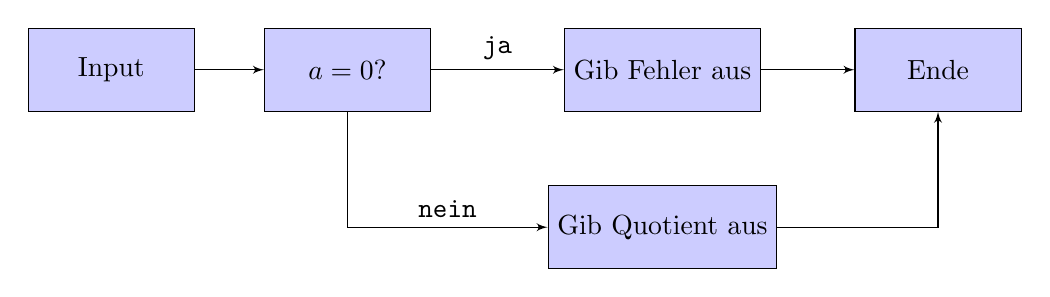
\begin{tikzpicture}[auto, node distance=3cm,>=latex']
        \tikzstyle{block} = [draw, fill=blue!20, rectangle, minimum height=3em, minimum width=6em]

        \node [block] (start) {Input};
        \node [block, right of=start] (if) { $a=0$? };
        \node [block, right of=if, node distance=4cm] (fehler) { Gib Fehler aus };
        \node [block, below of=fehler,node distance =  2cm] (quotient) { Gib Quotient aus };
        \node [block, right of=fehler, node distance = 3.5cm] (ende) { Ende };

        \draw [->] (start) -- node {} (if);
        \draw [->] (if) -- node {\texttt{ja}} (fehler);
        \draw [->] (if.south) |- node [above, near end] {\texttt{nein}} (quotient);
        \draw [->] (quotient) -| node {} (ende);
        \draw [->] (fehler) -- node {} (ende);
    \end{tikzpicture}
\end{center}

Die einfachste Möglichkeit, den Kontrollfluss zu ändern, besteht durch so
genannten „bedingten Anweisungen“:

\javasect{control/If.java}{11}{34}

In den Zeilen 21 bis 30 sehen wir, wie eine solche Bedingte Anweisung in \Java
aussieht. Wir erkennen relativ direkt unser Diagramm hier wieder: In Zeile 21
steht der „$b=0$?“ Block, in den Zeilen 22 bis 25 steht der „Gib Fehler aus“
Block und in den Zeilen 27 bis 28 der „Gib den Quotienten aus“ Block.

Beachtet allerding die doppelten Gleichheitszeichen „\verb|==|“ in Zeile
21. \Java hat getrennte Operatoren für Vergleiche und Zuweisungen -- Doppelte
Gleichheitszeichen bedeuten Vergleich („sind diese beiden gleich?“), ein
einfaches Gleichheitszeichen bedeutet Zuweisung („mache diese beiden gleich!“).

\textbf{Praxis:}
\begin{enumerate}
\item Kompiliert \texttt{If.java} für den Debugger und lasst das Programm im
  Debugger laufen. Geht Schritt für Schritt durch das Programm, mit
  verschiedenen Eingaben (wenn ihr am Ende des Programms angekommen seid, könnt
  ihr es erneut starten).
\item Nutzt Google, um herauszufinden, welche anderen Vergleichsoperatoren
  es in \Java noch gibt. Versucht, das Programm so zu verändern, dass es
  auf Ungleichheit testet, statt auf Gleichheit (sich sonst aber genauso
  verhält).
\item Wie würdet ihr testen, ob zwei Zahlen durch einander teilbar sind (Tipp:
  Ihr kennt bereits die Division mit Rest in \Java (modulo))? Schreibt ein
  Programm, welches zwei Zahlen von der Nutzerin entgegen nimmt und ausgibt, ob
  die zweite Zahl die erste teilt.
\end{enumerate}

\textbf{Spiel:}
\begin{enumerate}
\item Testet mit verschiedenen Eingaben, was passiert, wenn ihr in
  \texttt{If.java} statt zwei Gleichheitszeichen nur eines benutzt. Benutzt den
  Debugger, um euch den Inhalt von \texttt{b} vor und nach dem Test anzuschauen.
\item Schreibt ein Programm, welches die Benutzerin fragt, wie sie heißt. Gibt
  sie Euren eigenen Namen ein, soll das Programm begeistert über die
  Namensgleichheit sein, sonst die Nutzrin wie gewohnt begrüßen.
\end{enumerate}

\input{basics/schleifen}
\input{basics/style}
\lesson{Funktionen}

Wir haben den Begriff schon ein paarmal genannt und auch, wenn ihr es vielleicht
nicht gemerkt habt, sie waren schon die ganze Zeit vor eurer Nase: Funktionen.

Eine Funktion ist im Wesentlichen eine Möglichkeit, eine Folge von Anweisungen
zu bündeln und zu isolieren. Wir haben schon einmal ein Programm gesehen, mit
dem wir testen können, ob eine Zahl eine Primzahl ist, oder nicht. Viele
Vorteile von Funktionen, lassen sich an diesem Beispiel illustrieren. Stellt
euch vor, ihr braucht in eurem Programm an vielen Stellen einen solchen
Primzahltest. Ihr könntet jedes mal den gesamten benötigten Code hinschreiben,
aber das wäre doch eine Menge Arbeit. Eine Funktion ermöglicht es euch, den Code
für den Primzahltest in eine eigene Funktion auszulagern, nennen wir
sie \texttt{istPrim}. Immer, wenn Ihr dann testen wollt, ob eine Zahl \texttt{n}
eine Primzahl ist, könnt Ihr dann einfach schreiben \texttt{istprim(n)} und ruft
damit die Funktion auf. Das spart Schreibarbeit!

Stellt Euch vor, irgendwann ist Euch dann ein Test mittels Probedivision nicht
mehr schnell genug (weil ihr z.B. immer größere Zahlen testen wollt) und ihr
wollt auf einen schnelleren Test umsteigen. Ohne Funktionen müsstet ihr jedes
Vorkommen eines Primzahltests in Eurem Code einzeln durch den neuen Test
ersetzen. Mit Funktionen gibt es genau eine Stelle, an der Ihr den Code
austauschen müsst und all die Stellen, an denen ihr ihn benutzt, übernehmen
automatisch die neue Implementation.

Zuletzt haben wir in der letzten Lektion einiges über Lesbarkeit von Quellcode
gelernt. Lesbarkeit erhöht Wartbarkeit und reduziert die Möglichkeiten, Fehler
zu machen. Was stellt ihr Euch lesbarer vor, eine Datei, in der einige tausend
Zeilen Code stehen, einfach nur als Folge von Anweisungen ohne sichtbare
Struktur, oder mehrere kleine Datein, mit beschreibenden, verständlichen Namen,
in denen jeweils mehrere Funktionen, ebenfalls mit verständlichen Namen stehen,
das alles schön aufgeteilt nach Themengebieten? Funktionen erhöhen Lesbarkeit
und helfen, den Code zu strukturieren, was ihn verständlicher macht.

Das wohl wichtigste Beispiel für eine Funktion habt ihr bereits kennengelernt:
Die \texttt{main}-Funktion. Diese spezielle Funktion ist der Eintrittspunkt für
euer Programm. Der Code der \texttt{main}-Funktion ist der erste, der läuft,
sobald die \texttt{main} fertig abgearbeitet ist, beendet sich euer Programm.
Damit können wir an der \texttt{main} Funktion die wesentlichen Eckpunkte
ablesen, wie eine Funktion syntaktisch auszusehen hat.

Der Abschnitt
\begin{center}
  \texttt{public static void main(String[] args)}
\end{center}
heißt die \emph{Signatur} der Funktion. Wir ignorieren an dieser Stelle die
Schlüsselwörter \texttt{public} und \emph{static}. Die Signatur enthält immer
den Datentyp, den die Funktion ausgeben soll (in diesem Fall \texttt{void}, also
den „leeren Datentyp“. Diesen verwendet man, wenn keine Rückgabe einer Funktion
erwartet wird.), einen Namen (in diesem Fall der spezielle Name \texttt{main})
sowie Parameter, die Eingabewerte (in diesem Fall ein Parameter namens
\texttt{args} vom Datentyp \texttt{String[]}). An die Signatur schließt sich
direkt eine öffnende geschweifte Klammer, dann kommen alle Anweisungen, aus
denen die Funktion bestehen soll, dann eine schließende geschweifte Klammer.

Um das Ergebnis einer Funktion zurückzugeben, benutzen wir \texttt{return}. Wir
haben das bereits einmal gesehen, wo wir es benutzt haben, um unser Programm zu
beenden -- das funktionierte in dem Fall, weil wir uns in der \texttt{main}
befanden und wie gesagt, beendet sich das Programm, sobald die \texttt{main}
fertig ist. Mit Funktionen könnte ein Programm, was eine Zahl darauf testet,
eine Primzahl zu sein, so aussehen:

\javasect{funktionen/Funktion.java}{7}{46}

Parameter geben wir also in den Klammern an, jeweils so, wie wenn wir eine
Variable erstellen würden, mit einem Typ und einem Namen. Wenn wir mehrere
Parameter brauchen, können wir sie mit Kommata trennen. Dann müssen wir auch,
wenn wir die Funktion an anderer Stelle benutzen, die einzelnen Eingaben mit
Kommata trennen.

\textbf{Praxis:}
\begin{enumerate}
\item Schreibt eine Funktion, die einen Parameter vom Typ
  \texttt{String} hat und einen Rückgabewert vom Typ \texttt{int}. Die Funktion
  soll -- so wie wir es bisher schon in vielen Programmen gemacht haben -- den
  eingegebenen String (der z.B. die Aufforderung enthält, eine Zahl einzugeben)
  auf die Konsole ausgeben und einen \texttt{int} von der Nutzerin einlesen.
  Dieser eingelesene \texttt{int} soll dann von der Funktion zurückgegeben
  werden. Denkt euch einen sprechenden Namen für diese Funktion aus. (Ihr müsst
  vor die Angabe des Rückgabewertes die Schlüsselwörter \texttt{public static}
  schreiben und diese Voraussetzung zum jetzigen Zeitpunkt einfach so
  hinnehmen.)
\item Passt \texttt{Funktion.java} so an, dass es Eure Funktion benutzt.
\item Kompiliert das angepasste Programm und lasst es im Debugger Schritt für
  Schritt durchlaufen. Um die Funktion durchlaufen zu lassen, habt Ihr zwei
  Möglichkeiten: Ihr könnt einen neuen Breakpoint in der Funktion erstellen oder
  das Programm so lange Schritt für Schritt ablaufen, bin ihr in der Funktion
  angekommen seid.
\end{enumerate}

\textbf{Spiel:}
\begin{enumerate}
\item Vertauscht in \texttt{Funktion.java} die Funktion \texttt{istPrim} mit
  der Funktion \texttt{main} (verschiebt also die gesamte Funktion
  \texttt{istprim} an das Ende der Datei). Versucht, die Datei zu
  kompilieren. Was ist die Fehlermeldung des Compilers?
\item Verschiebt die Funktion \texttt{istPrim} \emph{in} die
  \texttt{main}-Funktion (also irgendwo nach der öffnenden geschweiften
  Klammern, aber vor die dazu gehörige schließende). Versucht, die Datei zu
  kompilieren. Was ist die Fehlermeldung des Compilers?
\item Schaut Euch Eure bisherigen Lösungen aus den anderen Kapiteln an. Findet ihr noch häufiger
  Stellen, an denen ihr einzelne Teilprogramme in Funktionen auslagern könnt?
\end{enumerate}

\input{basics/arrays}

\pagebreak
\pagestyle{empty}

\textbf{Herzlichen Glückwunsch!} Ihr habt diesen Selbstlernkurs zur Einführung
in die Programmierung (hoffentlich) erfolgreich durchgearbeitet.

Rekapitulieren wir noch einmal unsere Eingangs formulierten „Lernziele“, was
wir uns wünschen würden, dass ihr aus diesem Vorkurs mitnehmt:
\begin{itemize}
    \item Ein Computer ist keine schwarze Magie
    \item Programmieren ist keine schwarze Magie
    \item Ihr wisst, wo ihr anfangt, wenn die Aufgabe ist „schreibt ein
        Programm, das\dots“
    \item Ihr entwickelt Spaß daran, Programmieraufgaben zu lösen
    \item Ihr wisst, was ihr tun könnt, wenn etwas nicht funktioniert
\end{itemize}

Falls ihr bereits vorzeitig mit diesem Selbstlernkurs fertig seid, dann könnt
ihr Euch an folgenden Aufgaben probienen.

\begin{itemize}
\item Es soll ein Programm geschrieben werden, das alle geraden Zahlen von 1 bis 1000 ausgibt.
\item Es soll ein Programm geschrieben werden, das alle ungeraden Zahlen von 1 bis 1000 ausgibt.
\item Es soll ein Programm geschrieben werden, welches von der Nutzerin Gewicht
  und Größe abfragt und dann den Body Mass Index (BMI) ausgibt. Zusatz: Teile
  der Nutzerin auch mit, ob sie Über-, Unter oder Idealgewicht hat.
\end{itemize}


\end{document}
